\chapter{Diagrammi e risultati\label{sec:risultati}}
\noindent In questa sezione commentiamo alcuni diagrammi che illustrano i risultati ottenuti dai tre algoritmi implementati in termini di tempo a fronte della taglia del grafo.

\section{Diagrammi\label{sec:diagrammi}}

\begin{figure}[htp]
    \centering
    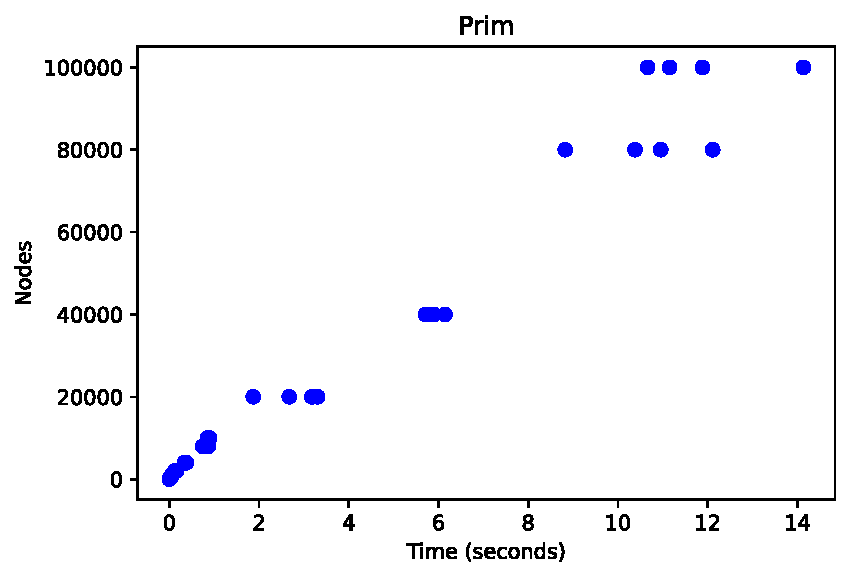
\includegraphics[width=\textwidth]{immagini/prim.pdf}
    \caption{Diagramma con tempi impiegati per Prim}
    \label{fig:diagramma-prim}
\end{figure}

\begin{figure}[htp]
    \centering
    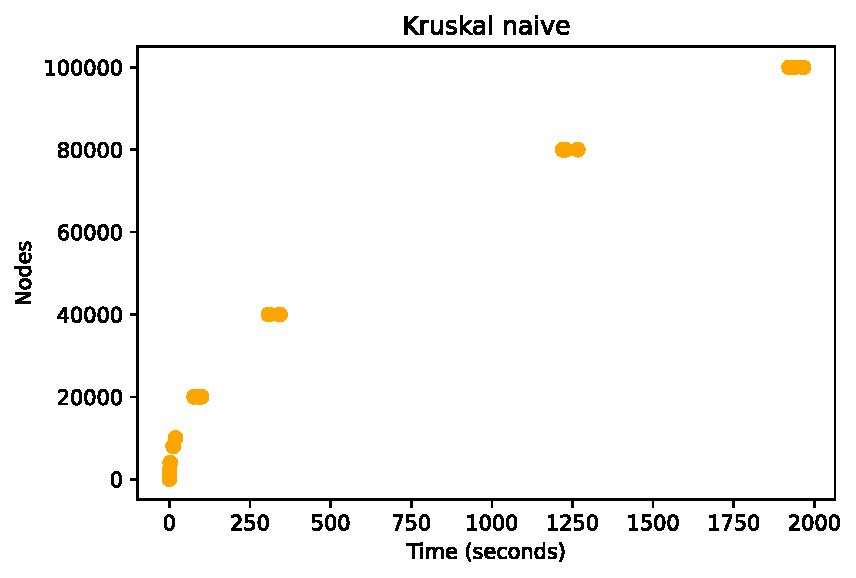
\includegraphics[width=\textwidth]{immagini/naive.pdf}
    \caption{Diagramma con tempi impiegati per Kruskal ``naive''}
    \label{fig:diagramma-naive}
\end{figure}

\begin{figure}[htp]
    \centering
    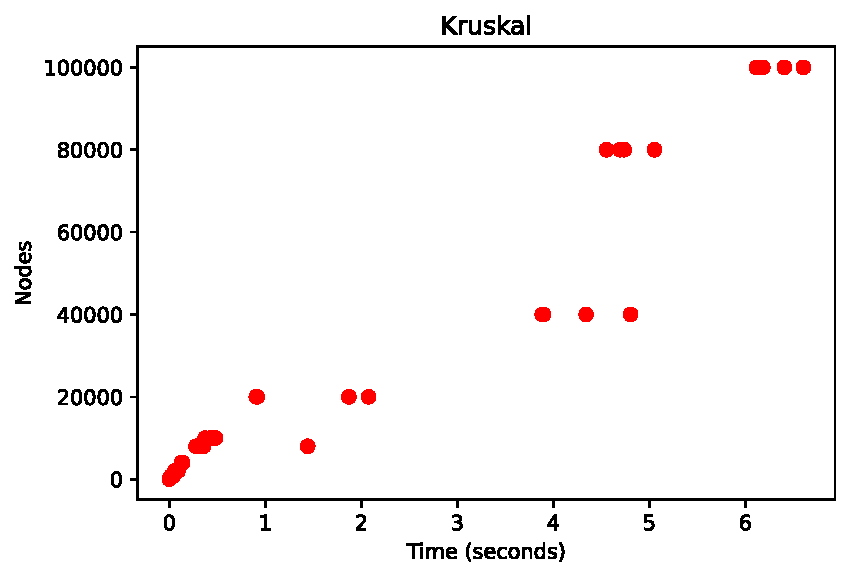
\includegraphics[width=\textwidth]{immagini/kruskal.pdf}
    \caption{Diagramma con tempi impiegati per Kruskal con Union-Find}
    \label{fig:diagramma-kruskal}
\end{figure}

\clearpage

\section{Risultati\label{sec:risultati}}
È chiaramente visibile dai diagrammi che rappresentano le tempistiche impiegate che Kruskal naive si comporta peggio rispetto agli altri algoritmi per la ricerca di un MST.
Questo conferma la complessità trovata a lezione, pari a O(mn), dove m è il numero di archi del grafo e n il numero di vertici.

Gli altri due algoritmi sono comparabili a livello di complessità, infatti i tempi impiegati sono dello stesso ordine di grandezza.

Pur essendo Prim e Kruskal con Union Find caratterizzati dalla stessa complessità computazionale (O(mlog(n))), per quanto misurato il secondo algoritmo si comporta meglio e impiega metà del tempo a parità di dimensione del grafo.
Questo potrebbe essere dovuto alla struttura usata per rappresentare il grafo (lista di adiacenza nel caso di Prim, lista di adiacenza e singoli lati nel caso di Kruskal con Union Find).